\documentclass[12pt]{article}
\usepackage[a4paper, margin=0.75in]{geometry}
\usepackage[document]{ragged2e}
\usepackage{graphicx}
\graphicspath{ {./images/} }
\usepackage{enumerate}
\usepackage{framed}
\usepackage{amsmath,amsfonts,amsthm,thmtools,amssymb,mathtools,commath}
\usepackage{physics}
\usepackage{tikz}
\usetikzlibrary{mindmap}
\usepackage{caption}
\usepackage{xcolor}
\usepackage[most]{tcolorbox}
\usepackage{cleveref}


%%%%%%%%%%%%%%%%
%  Definition  %
%%%%%%%%%%%%%%%%
\tcbuselibrary{theorems,skins,hooks}
\newtcbtheorem[number within=subsection]{definition}{Definition}%
{
    % theorem style=definition,
    enhanced,
	before skip=2mm,after skip=2mm, colback=cyan!5,colframe=cyan!80!black,boxrule=0.5mm,
	attach boxed title to top left={xshift=1cm,yshift*=1mm-\tcboxedtitleheight},
	boxed title style={frame code={
					\path[fill=cyan]
					([yshift=-1mm,xshift=-1mm]frame.north west)
					arc[start angle=0,end angle=180,radius=1mm]
					([yshift=-1mm,xshift=1mm]frame.north east)
					arc[start angle=180,end angle=0,radius=1mm];
					\path[left color=cyan!30!black,right color=cyan!30!black,
						middle color=cyan!50!black]
					([xshift=-2mm]frame.north west) -- ([xshift=2mm]frame.north east)
					[rounded corners=1mm]-- ([xshift=1mm,yshift=-1mm]frame.north east)
					-- (frame.south east) -- (frame.south west)
					-- ([xshift=-1mm,yshift=-1mm]frame.north west)
					[sharp corners]-- cycle;
				},interior engine=empty,
		},
	fonttitle=\bfseries,
	title={#2},#1
}{def}


%%%%%%%%%%%%%
%  Theorem  %
%%%%%%%%%%%%%
\tcbuselibrary{theorems,skins,hooks}
\newtcbtheorem[use counter from=definition]{theorem}{Theorem}%
{
    theorem style=plain,
    enhanced,
    colframe=green,
    boxrule=1pt,
    titlerule=0mm,
    toptitle=1mm,
    bottomtitle=1mm,
    fonttitle=\bfseries,
    fontupper=\mdseries\itshape,
    coltitle=green!30!black,
    colbacktitle=cyan!15!white,
    colback=green!10,
    description font=\bfseries\sffamily
}{thrm}


%%%%%%%%%%%%%%
% Corollary  %
%%%%%%%%%%%%%%
 \tcbuselibrary{theorems,skins}
 \newtcbtheorem[use counter from=theorem]{corollary}{Corollary}%
 {
    theorem style=plain,
    enhanced,
    colframe=green,
    frame hidden,
    titlerule=0mm,
    toptitle=1mm,
    bottomtitle=1mm,
    fonttitle=\bfseries,
    fontupper=\mdseries\itshape,
    coltitle=green!30!black,
    colbacktitle=cyan!15!white,
    colback=green!10,
    description font=\bfseries\sffamily
 }{corl}


%%%%%%%%%%%%%
%  Example  %
%%%%%%%%%%%%%
\tcbuselibrary{theorems,skins,hooks}
\newtcbtheorem[number within=section]{example}{Example}%
{
	enhanced,
	breakable,
	colback = gray!5,
	frame hidden,
	boxrule = 0sp,
	borderline west = {2pt}{0pt}{gray},
	sharp corners,
	detach title,
	before upper = \tcbtitle\par\smallskip,
    coltitle=gray!70!black,
	fonttitle = \bfseries\sffamily,
	description font = \mdseries\bfseries
}
{xmp}


%%%%%%%%%%%%%%
%  Exercise  %
%%%%%%%%%%%%%%
\tcbuselibrary{theorems,skins,hooks}
\newtcbtheorem[number within=section]{exercise}{Exercise}%
{
    enhanced,
    breakable,
    colback=black!5,
    colframe=black!30,
    left=0.5em,
    before skip=10pt,
    after skip=10pt,
    boxrule=0pt,
    boxsep=0pt,
    arc=0pt,
    outer arc=0pt,
    borderline west={3pt}{0pt}{black!30},
}{exc}

%%%%%%%%%%
%  Note  %
%%%%%%%%%%
\usetikzlibrary{arrows,calc,shadows.blur}
\tcbuselibrary{skins}
\newtcolorbox{note}[1][]{%
	enhanced jigsaw,
	colback=gray!20!white,%
	colframe=gray!80!black,
	size=small,
	boxrule=1pt,
	title=\textbf{Note:-},
	halign title=flush center,
	coltitle=black,
	breakable,
	drop shadow=black!50!white,
	attach boxed title to top left={xshift=1cm,yshift=-\tcboxedtitleheight/2,yshifttext=-\tcboxedtitleheight/2},
	minipage boxed title=1.5cm,
	boxed title style={%
			colback=white,
			size=fbox,
			boxrule=1pt,
			boxsep=2pt,
			underlay={%
					\coordinate (dotA) at ($(interior.west) + (-0.5pt,0)$);
					\coordinate (dotB) at ($(interior.east) + (0.5pt,0)$);
					\begin{scope}
						\clip (interior.north west) rectangle ([xshift=3ex]interior.east);
						\filldraw [white, blur shadow={shadow opacity=60, shadow yshift=-.75ex}, rounded corners=2pt] (interior.north west) rectangle (interior.south east);
					\end{scope}
					\begin{scope}[gray!80!black]
						\fill (dotA) circle (2pt);
						\fill (dotB) circle (2pt);
					\end{scope}
				},
		},
	#1,
}

\usepackage{makecell}
\allowdisplaybreaks
\numberwithin{equation}{subsection}

\title{
    \textbf{Simple Harmonic Motion and Waves}
}

\author{
    Turja Roy\\
    ID: 2108052
}
\date{}

\begin{document}
\maketitle
\tableofcontents
\newpage

\section{Oscillation and Vibration}
\subsection{Oscillation}
\begin{itemize}
    \item Oscillation is the repetitive variation, typically in time, of some measure about a central value (often a point of equilibrium) or between two or more different states.
    \item The term vibration is precisely used to describe mechanical oscillation.
    \item Familiar examples of oscillation include a swinging pendulum and alternating current.
\end{itemize}

\subsection{Vibration}
\begin{itemize}
    \item Vibration is a mechanical phenomenon whereby oscillations occur about an equilibrium point.
    \item The word comes from Latin vibrationem ("shaking, brandishing").
    \item The oscillations may be periodic, such as the motion of a pendulum—or random, such as the movement of a tire on a gravel road.
\end{itemize}

\subsection{Differences between Oscillation and Vibration}
\begin{itemize}
    \item Oscillation is the definite displacement of a body in terms of distance or time, whereas vibration is the movement brought about in a body due to oscillation.
    \item Oscillation takes place in physical, biological systems, and often in our society, but vibrations is associated with mechanical systems only.
    \item Oscillation is about a single body, whereas vibration is the result of collective oscillation of atoms in the body.
    \item All vibrations are oscillations, but not all oscillations are vibrations.
\end{itemize}

\section{Simple Harmonic Motion}
\subsection{Definition}

\begin{definition}{Simple Harmonic Motion}{}
    Simple harmonic motion is a type of periodic motion where the restoring force is directly proportional to the displacement and acts in the direction opposite to that of displacement.
\end{definition}

A particle is said to execute SHM when it will
\begin{enumerate}[(a)]
    \item Trace and retrace the same path over and over again.
    \item Change direction at a regular interval of time.
    \item Move along a straight line.
    \item Have acceleration proportional to its displacement from the mean position.
\end{enumerate}

A particle which satisfies the condition (a) only is said to execute \textbf{periodic motion}. A particle which satisfies condition (a) and (b) is said to execute \textbf{vibratory motion}. \\~\\

Let $P$ be a particle moving on the circumference of a circle of radius $r$ with a uniform velocity $v$. Let angular velocity be $\omega = v/r$.

\begin{figure}[htpb]
    \centering
    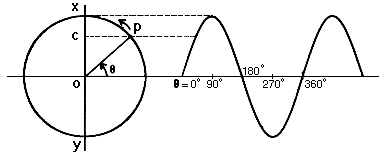
\includegraphics[width=0.5\textwidth]{1.png}
\end{figure}

\vspace{20pt}
Displacement of the particle from the mean position is given by $\displaystyle y = r \sin{\omega t}$\\
So, velocity of the particle is given by $\displaystyle v = \frac{dy}{dt} = \omega r \cos{\omega t}$\\
And acceleration of the particle is given by $\displaystyle a = \frac{dv}{dt} = -\omega^2 r \sin{\omega t} = -\omega^2 y$

\vspace{20pt}
\begin{center}
    \begin{tabular}{c | c | c | c | c}
        Angle & \makecell{Position of \\ vibrating particle} & \makecell{Displacement \\ $y = r \sin{\omega t}$} & \makecell{Velocity \\ $\displaystyle \dv{y}{t} = \omega r \cos{\omega t}$} & \makecell{Acceleration \\ $-\omega^2 r \sin{\omega t} = -\omega^2 y$} \\\hline\hline
        0 & O & 0 & $\omega r$ & 0 \\\hline
        $\pi/2$ & X & $r$ & 0 & $-\omega^2 a$ \\\hline
        $\pi$ & O & 0 & $-\omega r$ & 0 \\\hline
        $3\pi/2$ & Y & $-r$ & 0 & $\omega^2 r$ \\\hline
        $2\pi$ & O & 0 & $\omega r$ & 0
    \end{tabular}
\end{center}

\subsection{Differential Equation of SHM}
Let $y$ be the displacement of the particle from the mean position at time $t$, $r$ be the amplitude, and $\alpha$ be the epoch of the vibrating particle \\
\begin{equation}
    y = r \sin{(\omega t + \alpha)}
\end{equation}
\begin{equation}
    \dv{y}{t} = r \omega \cos{(\omega t + \alpha)}
\end{equation}
\begin{equation}
    \dv[2]{y}{t} = -r \omega^2 \sin{(\omega t + \alpha)}
\end{equation}

Hence the differential equation of SHM is
\begin{equation}
    \dv[2]{y}{t} + \omega^2 y = 0
\end{equation}

\subsection{Solution of the Differential Equation of SHM}
\begin{equation}
    \dv[2]{y}{t} + \omega^2 y = 0
\end{equation}

Here, \[
    \dv[2]{y}{t} = \dv{v}{t} = \dv{v}{y} \dv{y}{t} = v \dv{v}{y}
\]
\begin{align*}
    v \: d{v} + \omega^2y \: d{y} &= 0 \\
    \int{v} \: d{v} + \omega^2 \int{y} \: d{y} &= 0 \\
    \frac{v^2}{2} + \frac{\omega^2 y^2}{2} &= C' \\
    \left( \dv{y}{t} \right) ^2 + \omega^2 y^2 &= C^2
\end{align*}

At maximum displacement, $y = r$ and $\displaystyle \dv{y}{t} = 0$ \\
So, $C^2 = \omega^2 r^2$ \\
\begin{align*}
    \left( \dv{y}{t} \right)^2 &= \omega^2(r^2 - y^2) \\
    \dv{y}{t} &= \omega \sqrt{r^2 - y^2} \\
    \int{\frac{1}{\sqrt{r^2-y^2}}} \: d{y} &= \int{\omega} \: d{t} \\
    \sin^{-1}{\frac{y}{r}} &= \omega t + \alpha
\end{align*}
\begin{equation}
    \boxed{ y = r \sin{(\omega t + \alpha)} }
\end{equation}

By expanding equation (2.3.2), we get
\begin{equation}
    y = r \sin{\omega t} \cos{\alpha} + r \cos{\omega t} \sin{\alpha}
\end{equation}
If $y = 0$ at $t = 0$, then $\alpha = 0$ \\
\begin{equation}
    y = r \sin{\omega t}
\end{equation}
If $y = r$ at $t = 0$, then $\alpha = \pi/2$ \\
\begin{equation}
    y = r \cos{\omega t}
\end{equation}

Hence, the general solution of the differential equation of SHM is
\begin{equation}
    \boxed{ y = A \sin{\omega t} + B \cos{\omega t} }
\end{equation}

\section{Energy in SHM}
\subsection{Total Energy of a Vibrating Particle}
\begin{align*}
    \text{Kinetic Energy} &= \frac{1}{2} m \left( \dv{y}{t} \right)^2 \\
    &= \frac{1}{2} m \omega^2 r^2 \cos^2{(\omega t + \alpha)} \\
    \text{Potential Energy} &= \frac{1}{2} k y^2 \\
    &= \frac{1}{2} m \omega^2 r^2 \\
    &= \frac{1}{2} m \omega^2 r^2 \sin^2{(\omega t + \alpha)}
\end{align*}

Thus, the total energy of the vibrating particle is
\begin{equation}
    \boxed{ E = \frac{1}{2} k r^2 = \frac{1}{2} m \omega^2 r^2 }
\end{equation}

\begin{figure}[htpb]
    \centering
    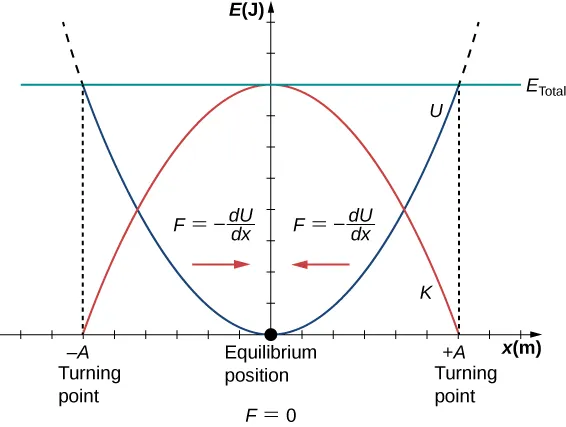
\includegraphics[width=0.5\textwidth]{2.png}
\end{figure}

\subsection{Average Kinetic Energy}
Kinetic energy of the particle is given by
\begin{equation}
    K = \frac{1}{2} m \left( \dv{y}{t} \right)^2 = \frac{1}{2} m \omega^2 r^2 \cos^2{(\omega t + \alpha)}
\end{equation}
Hence, average kinetic energy is
\begin{align*}
    \overline{K} &= \frac{1}{T} \int_{0}^{T} K \: dt \\
    &= \frac{1}{T} \int_{0}^{T} \frac{1}{2} m \omega^2 r^2 \cos^2{(\omega t + \alpha)} \: dt \\
    &= \frac{1}{2} m \omega^2 r^2 \frac{1}{T} \int_{0}^{T} \cos^2{(\omega t + \alpha)} \: dt \\
    &= \frac{1}{2} m \omega^2 r^2 \frac{1}{T} \int_{0}^{T} \frac{1 + \cos{2(\omega t + \alpha)}}{2} \: dt \\
    &= \frac{1}{2} m \omega^2 r^2 \frac{1}{T} \left[ \frac{t}{2} + \frac{\sin{2(\omega t + \alpha)}}{4\omega} \right]_{0}^{T} \\
    &= \frac{1}{2} m \omega^2 r^2 \frac{1}{T} \left[ \frac{T}{2} + \frac{\sin{2(\omega T + \alpha)}}{4\omega} - \frac{\sin{2\alpha}}{4\omega} \right] \\
    &= \frac{1}{2} m \omega^2 r^2 \frac{1}{T} \left[ \frac{T}{2} + \frac{\sin{2\alpha}}{4\omega} - \frac{\sin{2\alpha}}{4\omega} \right] \\
    &= \frac{1}{4} m \omega^2 r^2
\end{align*}
\begin{equation}
    \boxed{ \overline{K} = \frac{1}{4} m \omega^2 r^2 = \frac{1}{4}k r^2 = \frac{1}{2} E }
\end{equation}

\subsection{Average Potential Energy}
Potential energy of the particle is given by
\begin{equation}
    U = \frac{1}{2} k y^2 = \frac{1}{2} m \omega^2 r^2 \sin^2{(\omega t + \alpha)}
\end{equation}
Hence, average potential energy is
\begin{align*}
    \overline{U} &= \frac{1}{T} \int_{0}^{T} U \: dt \\
    &= \frac{1}{T} \int_{0}^{T} \frac{1}{2} m \omega^2 r^2 \sin^2{(\omega t + \alpha)} \: dt \\
    &= \frac{1}{2} m \omega^2 r^2 \frac{1}{T} \int_{0}^{T} \sin^2{(\omega t + \alpha)} \: dt \\
    &= \frac{1}{2} m \omega^2 r^2 \frac{1}{T} \int_{0}^{T} \frac{1 - \cos{2(\omega t + \alpha)}}{2} \: dt \\
    &= \frac{1}{2} m \omega^2 r^2 \frac{1}{T} \left[ \frac{t}{2} - \frac{\sin{2(\omega t + \alpha)}}{4\omega} \right]_{0}^{T} \\
    &= \frac{1}{2} m \omega^2 r^2 \frac{1}{T} \left[ \frac{T}{2} - \frac{\sin{2(\omega T + \alpha)}}{4\omega} + \frac{\sin{2\alpha}}{4\omega} \right] \\
    &= \frac{1}{2} m \omega^2 r^2 \frac{1}{T} \left[ \frac{T}{2} + \frac{\sin{2\alpha}}{4\omega} - \frac{\sin{2\alpha}}{4\omega} \right] \\
    &= \frac{1}{4} m \omega^2 r^2
\end{align*}
\begin{equation}
    \boxed{ \overline{U} = \frac{1}{4} m \omega^2 r^2 = \frac{1}{4}k r^2 = \frac{1}{2} E }
\end{equation}

\section{Composition of Two SHMs of Same Frequency}
\subsection{Same Direction}

Let $y_1$ and $y_2$ be the displacements of two SHM of same frequency $\omega$, amplitude $r_1$ and $r_2$, and phases $\alpha_1$ and $\alpha_2$ respectively. \\
\begin{align}
    y_1 &= r_1 \sin{(\omega t + \alpha_1)} \\
    y_2 &= r_2 \sin{(\omega t + \alpha_2)}
\end{align}

If the two SHMs are in the same direction, then the resultant displacement is
\begin{align*}
    y &= y_1 + y_2 \\
    &= r_1 \sin{(\omega t + \alpha_1)} + r_2 \sin{(\omega t + \alpha_2)} \\
    &= r_1 \sin{\omega t} \cos{\alpha_1} + r_1 \cos{\omega t} \sin{\alpha_1} + r_2 \sin{\omega t} \cos{\alpha_2} + r_2 \cos{\omega t} \sin{\alpha_2}
\end{align*}
\begin{equation}
    \therefore y = (r_1 \cos{\alpha_1} + r_2 \cos{\alpha_2}) \sin{\omega t} + (r_1 \sin{\alpha_1} + r_2 \sin{\alpha_2}) \cos{\omega t}
\end{equation}

In equation (4.1.3), let
\begin{align}
    r_1\cos{\alpha_1} + r_2\cos{\alpha_2} &= A\cos{\varphi} \\
    r_1\sin{\alpha_1} + r_2\sin{\alpha_2} &= A\sin{\varphi}
\end{align}

Then, equation (4.1.3) becomes
\begin{align}
    y &= A\cos{\varphi} \sin{\omega t} + A\sin{\varphi} \cos{\omega t} \\
    y &= A \sin{(\omega t + \varphi)}
\end{align}

Here, $A$ is the amplitude of the resultant SHM and $\varphi$ is the phase of the resultant SHM. \\

From equations (4.1.4) and (4.1.5), we get
\begin{align*}
    A^2 &= A^2 \sin^2{\varphi} + A^2 \cos^2{\varphi} \\
    A^2 &= 
    \begin{aligned}[t]
        & r_1^2 \sin^2{\alpha_1} + r_2^2 \sin^2{\alpha_2} + 2r_1r_2 \sin{\alpha_1} \sin{\alpha_2} \\
            & + r_1^2 \cos^2{\alpha_1} + r_2^2 \cos^2{\alpha_2} + 2r_1r_2 \cos{\alpha_1} \cos{\alpha_2}
    \end{aligned}\\
    A^2 &= r_1^2 + r_2^2 + 2r_1r_2(\sin{\alpha_1} \sin{\alpha_2} + \cos{\alpha_1} \cos{\alpha_2}) \\
    A^2 &= r_1^2 + r_2^2 + 2r_1r_2 \cos{(\alpha_1 - \alpha_2)}
\end{align*}

\begin{equation}
    \boxed{ A = \sqrt{r_1^2 + r_2^2 + 2r_1r_2 \cos{(\alpha_1 - \alpha_2)}} }
\end{equation}

And,
\begin{equation}
    \boxed{ \varphi = \tan^{-1}{\frac{r_1 \sin{\alpha_1} + r_2 \sin{\alpha_2}}{r_1 \cos{\alpha_1} + r_2 \cos{\alpha_2}}} }
\end{equation}

\subsubsection{Special Cases}
\textbf{(I) Same phase : $\alpha_1 = \alpha_2$}\\~\\

In this case, equation (4.1.8) becomes \[
    A = \sqrt{r_1^2 + r_2^2 + 2r_1r_2 \cos{0}} = \sqrt{(r_1 + r_2)^2} = r_1 + r_2
\]
\begin{equation}
    \boxed{ A = r_1 + r_2 }
\end{equation}

And, \[
    \varphi = \tan^{-1}{\frac{r_1 \sin{\alpha} + r_2 \sin{\alpha}}{r_1 \cos{\alpha} + r_2 \cos{\alpha}}} = \tan^{-1}{\left( \frac{r_1 + r_2}{r_1 + r_2} \tan{\alpha} \right)} = \tan^{-1}{(\tan{\alpha})}
\]
\begin{equation}
    \boxed{ \varphi = \alpha }
\end{equation}

\textbf{(II) Opposite phase : $\alpha_1 - \alpha_2 = (2n+1)\pi \text{, where } n=0,1,2,\cdots$}

In this case, equation (4.1.8) becomes \[
    A = \sqrt{r_1^2 + r_2^2 + 2r_1r_2 \cos{(\alpha_2 + \pi - \alpha_2)}} = \sqrt{(r_1 - r_2)^2} = r_1 - r_2
\]
\begin{equation}
    \boxed{ A = r_1 - r_2 }
\end{equation}

And, \[
    \varphi = \tan^{-1}{\frac{r_1 \sin{(\alpha + \pi)} + r_2 \sin{\alpha}}{r_1 \cos{(\alpha + \pi)} + r_2 \cos{\alpha}}} = \tan^{-1}{\left( \frac{r_1 \sin{\alpha} - r_2 \sin{\alpha}}{r_1 \cos{\alpha} - r_2 \cos{\alpha}} \right)} = \tan^{-1}{(-\tan{\alpha})}
\]
\begin{equation}
    \boxed{ \varphi = \alpha + \pi }
\end{equation}


\subsection{Right Angle}
Let $x$ and $y$ be the displacements of two SHM of same frequency $\omega$, amplitude $a$ and $b$ respectively, and phase difference $\alpha$, acting at right angle to each other. \\
\begin{align}
    x &= a \sin{(\omega t + \alpha)} \\
    y &= b \sin{(\omega t)}
\end{align}
Or,
\begin{align}
    \frac{x}{a} &= \sin{(\omega t + \alpha)} \\
    \frac{y}{b} &= \sin{(\omega t)}
\end{align}

Thus, we get
\begin{align*}
    \frac{x}{a} &= \sin{\omega t}\cos{\alpha} + \cos{\omega t}\sin{\alpha} \\
    \frac{x}{a} &= \frac{y}{b} \sqrt{1 - \sin^2{\alpha}} + \sqrt{1 - \frac{y^2}{b^2}} \sin{\alpha} \\
    \frac{x}{a} - \frac{y}{b} \sqrt{1 - \sin^2{\alpha}} &= \sqrt{1 - \frac{y^2}{b^2}} \sin{\alpha} \\
    \frac{x^2}{a^2} + \frac{y^2}{b^2} (1 - \sin^2{\alpha}) - \frac{2xy}{ab} \sqrt{1 - \sin^2{\alpha}} &= \left( 1 - \frac{y^2}{b^2} \right) \sin^2{\alpha}
\end{align*}
\begin{equation}
    \boxed{ \frac{x^2}{a^2} + \frac{y^2}{b^2} - \frac{2xy}{ab} \sqrt{1 - \sin^2{\alpha}} = \sin^2{\alpha} }
\end{equation}

Equation (4.2.5) represents the general equation of the resultant SHM of the two perpendicular SHMs. The resulting curves are also known as Lissajous firgures.

\subsubsection{Special Cases}
\textbf{(I) If $\alpha=0$ or $2\pi$}\\~\\
\[ \cos{\alpha} = 1, \qquad \sin{\alpha} = 0 \]
Then equation (4.2.5) becomes \[
    \frac{x^2}{a^2} + \frac{y^2}{b^2} - \frac{2xy}{ab} = 0
\]
Or, \[
    \frac{x}{a} = \frac{y}{b}
\]
This represents a straight line passing through the origin.\\~\\


\textbf{(II) If $\alpha=\pi$}\\~\\
\[ \cos{\alpha} = -1, \qquad \sin{\alpha} = 0 \]
Then equation (4.2.5) becomes \[
    \frac{x^2}{a^2} + \frac{y^2}{b^2} + \frac{2xy}{ab} = 0
\]
Or, \[
    \frac{x}{a} = -\frac{y}{b}
\]
This represents a straight line with negative slope passing through the origin.\\~\\


\textbf{(III) If $\alpha=\pi/2$ or, $3\pi/2$}\\~\\
\[ \cos{\alpha} = 0, \qquad \sin{\alpha} = 1 \]
Then equation (4.2.5) becomes \[
    \frac{x^2}{a^2} + \frac{y^2}{b^2} = 1
\]
This represents an ellipse.\\~\\

\textbf{(IV) If $\alpha=\pi/2$ or, $3\pi/2$, and $a=b$}\\~\\
\[ \cos{\alpha} = 0, \qquad \sin{\alpha} = 1 \]
Then equation (4.2.5) becomes \[
    \frac{x^2}{a^2} + \frac{y^2}{a^2} = 1
\]
Or, \[
    x^2 + y^2 = a^2
\]
This represents a circle of radius $a$.\\~\\

\textbf{(V) If $\alpha=\pi/4$ or, $7\pi/4$}\\~\\
\[ \cos{\alpha} = \frac{1}{\sqrt{2}}, \qquad \sin{\alpha} = \frac{1}{\sqrt{2}} \]
Then equation (4.2.5) becomes \[
    \frac{x^2}{a^2} + \frac{y^2}{b^2} - \frac{2xy}{ab} \frac{1}{\sqrt{2}} = \frac{1}{2}
\]
This represents an oblique ellipse.\\~\\

\textbf{(VI) If $\alpha=3\pi/4$ or, $5\pi/4$}\\~\\
\[ \cos{\alpha} = -\frac{1}{\sqrt{2}}, \qquad \sin{\alpha} = \frac{1}{\sqrt{2}} \]
Then equation (4.2.5) becomes \[
    \frac{x^2}{a^2} + \frac{y^2}{b^2} + \frac{2xy}{ab} \frac{1}{\sqrt{2}} = \frac{1}{2}
\]
This represents an oblique ellipse (negative slope).\\~\\

\begin{figure}[htpb]
    \centering
    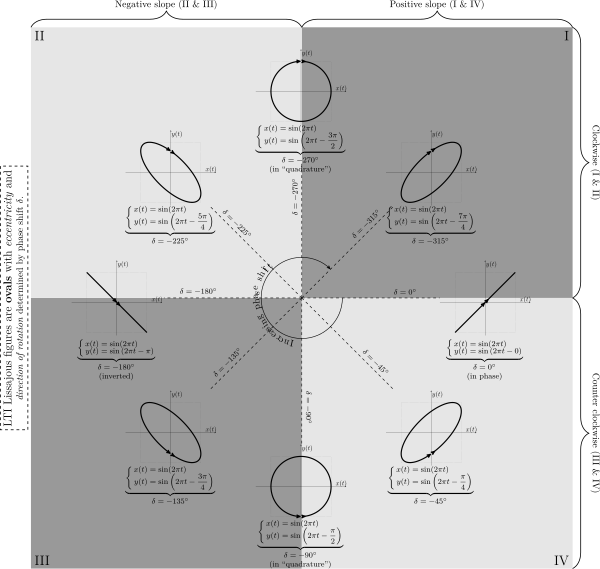
\includegraphics[width=0.9\textwidth]{Lissajous.png}
    \caption{Lissajous figures}
    \label{fig:Lissajous-png}
\end{figure}
\newpage

\section{Damped Harmonic Motion}
\subsection{Definition}

\begin{definition}{Damped Harmonic Motion}{}
    Damped harmonic motion is a type of periodic motion where the amplitude of the motion decreases over time.
\end{definition}

\begin{definition}{Damping and Damped Oscillation}{}
    Damping is an influence within or upon an oscillatory system that has the effect of reducing, restricting or preventing its oscillations. In physical systems, damping is produced by processes that dissipate the energy stored in the oscillation. \\
    In other words, the reduction in amplitude (or energy) of an oscillator is called damping, and the oscillation is said to be damped
\end{definition}

\begin{definition}{Damping Force}{}
    Damping force is a force, that opposes the motion of the vibrating particle and is directly proportional to the velocity of the particle.
    \begin{itemize}
        \item The damping force is always directed opposite to the direction of motion of the particle.
        \item The magnitude of the damping force is directly proportional to the velocity of the particle.
        \item The direction of the damping force is opposite to the direction of the velocity of the particle.
        \item Damping force is defined as $F_d = -bv$, where $b$ is the damping constant, and $v$ is the velocity of the object.
    \end{itemize}
\end{definition}

\subsection{Differential Equation of Damped Harmonic Motion}
The damping force can be represented as \[
    F_d = -bv = -b \dv{y}{t}
\]

Thus, the differential equation can be written as
\begin{align*}
    m \dv[2]{y}{t} &= -ky -b\dv{y}{t} \\
    m \dv[2]{y}{t} + b\dv{y}{t} + ky &= 0 \\
    \dv[2]{y}{t} + \frac{b}{m}\dv{y}{t} + \frac{k}{m}y &= 0
\end{align*}
\begin{equation}
    \boxed{ \dv[2]{y}{t} + 2\lambda \dv{y}{t} + \omega^2 y = 0 }
\end{equation}

Here, $\displaystyle \lambda = \frac{b}{2m}$ and $\displaystyle \omega = \sqrt{\frac{k}{m}}$ \\



\subsection{Solution of the Differential Equation}
Equation (5.1.1) is a second order linear differential equation with constant coefficients. So, it must have at least one solution of the form \[
    y = A e^{kt}
\]
, where $A$ and $k$ are arbitrary constants.\\
Hence, the auxiliary equation would be
\begin{equation}
    k^2 + 2\lambda k + \omega^2 = 0
\end{equation}
Equation (5.1.2) is a quadratic equation in $k$. So, it has two roots \[
    k = -\lambda \pm \sqrt{\lambda^2 - \omega^2}
\]

Thus, the general solution of the differential equation is
\begin{equation}
    \boxed{ y = A_1 e^{(-\lambda + \sqrt{\lambda^2 - \omega^2})t} + A_2 e^{(-\lambda - \sqrt{\lambda^2 - \omega^2})t} }
\end{equation}
Here, $A_1$ and $A_2$ are arbitrary constants. \\
Differentiating equation (5.1.3) with respect to $t$, we get
\begin{equation}
    \dv{y}{t} = (-\lambda + \sqrt{\lambda^2 - \omega^2})A_1 e^{(-\lambda + \sqrt{\lambda^2 - \omega^2})t} + (-\lambda - \sqrt{\lambda^2 - \omega^2})A_2 e^{(-\lambda - \sqrt{\lambda^2 - \omega^2})t}
\end{equation}

Let $y_{max} = a_0$ at $t=0$. Then, equation (5.3.3) becomes
\begin{equation}
    y_{max} = a_0 = A_1 + A_2
\end{equation}
Again, the velocity is zero at maximum displacement. So, equation (5.3.3) becomes
\begin{align*}
    \left( -\lambda + \sqrt{\lambda^2-\omega^2} \right) A_1 + \left( -\lambda - \sqrt{\lambda^2-\omega^2} \right) &= 0 \\
    - \lambda (A_1+A_2) + \sqrt{\lambda^2-\omega^2} (A_1-A_2) &= 0 \\
    - \lambda a_0 + \sqrt{\lambda^2-\omega^2} (A_1-A_2) &= 0 \\
    \sqrt{\lambda^2-\omega^2} (A_1-A_2) &= \lambda a_0
\end{align*}
\begin{equation}
    A_1 - A_2 = \frac{\lambda a_0}{\sqrt{\lambda^2-\omega^2}}
\end{equation}

From equations (5.3.4) and (5.3.5), we get
\begin{align}
    A_1 &= \frac{a_0}{2} \left( 1 + \frac{\lambda}{\sqrt{\lambda^2-\omega^2}} \right) \\
    \text{And}, \quad A_2 &= \frac{a_0}{2} \left( 1 - \frac{\lambda}{\sqrt{\lambda^2-\omega^2}} \right)
\end{align}

Substituting the values of $A_1$ and $A_2$ in equation (5.1.3), we get
\begin{equation}
    \boxed{ y = \frac{a_0}{2} e^{-\lambda t} \left[ \left( 1 + \frac{\lambda}{\sqrt{\lambda^2-\omega^2}} \right) e^{\sqrt{\lambda^2-\omega^2}t} + \left( 1 - \frac{\lambda}{\sqrt{\lambda^2-\omega^2}} \right) e^{-\sqrt{\lambda^2-\omega^2}t} \right] }
\end{equation}

\subsection{Over Damping, Critical Damping, and Under Damping}
\subsubsection{Over Damping}
When $\lambda > \omega$, then $\sqrt{\lambda^2-\omega^2}$ is a positive value, less than $\lambda$. Thus, each of the two terms on the RHS of equation (5.3.8) has exponential terms with negative power. In this case, the equation has no oscillating terms. So, the displacement falls asymptotically to zero without oscillating.

\subsubsection{Critical Damping}
When $\lambda = \omega$, then $\sqrt{\lambda^2-\omega^2} = 0$. Thus, the two terms on the RHS of equation (5.3.8) become \[
    \frac{a_0}{2} e^{-\lambda t} \left[ \left( 1 + \frac{\lambda}{\sqrt{\lambda^2-\omega^2}} \right) + \left( 1 - \frac{\lambda}{\sqrt{\lambda^2-\omega^2}} \right) \right] = a_0 e^{-\lambda t}
\]
In this case, the displacement falls asymptotically to zero without oscillating in the shortest possible time. \\~\\

Let's consider, however, that $\lambda^2 \to \omega^2$. Let $\sqrt{\lambda^2-\omega^2} = h$, a very small quantity. Then we have
\begin{align*}
    y &= A_1e^{(-\lambda+h)t} + A_2e^{(-\lambda-h)t} \\
    &= e^{-\lambda t} \left[ A_1e^{ht} + A_2e^{-ht} \right] \\
    &= e^{-\lambda t} \left[ A_1(1+ht+\frac{h^2t^2}{2!}+\cdots) + A_2(1-ht+\frac{h^2t^2}{2!}-\cdots) \right] \\
    &= e^{-\lambda t} \left[ (A_1+A_2) + (A_1-A_2)ht + \frac{h^2t^2}{2!}(A_1+A_2) + \cdots \right]
\end{align*}
We have $A_1 + A_2 = a_0$ and $\displaystyle A_1 - A_2 = \frac{\lambda a_0}{h} \qquad \text{[From equation (5.3.5)]}$ \\
Neglecting the higher powers of $h$, we get
\begin{equation}
    \boxed{ y = a_0 e^{-\lambda t} (1 + \lambda t) }
\end{equation}

This is the equation of motion of a critically damped oscillator. \\

\subsubsection{Under Damping}
When $\lambda < \omega$, then $\sqrt{\lambda^2-\omega^2}$ is an imaginary value. Let $i=\sqrt{-1}$ and $g=\sqrt{\omega^2-\lambda^2}$. So, equation (5.3.8) becomes
\begin{align*}
    y &= A_1e^{(-\lambda+ig)t} + A_2e^{(-\lambda-ig)t} \\
    &= e^{-\lambda t} (A_1e^{igt} + A_2e^{-igt}) \\
    &= e^{-\lambda t} \left[ A_1(\cos{gt}+i\sin{gt}) + A_2(\cos{gt}-i\sin{gt}) \right] \\
    &= e^{-\lambda t} \left[ (A_1+A_2)\cos{gt} + i(A_1-A_2)\sin{gt}\right ] \\
    y &= e^{-\lambda t} \left[ A \cos{gt} + B \sin{gt} \right]
\end{align*}

If $A$ and $B$ can be related to $a_0$ as $A = a_0\sin{\theta}$ and $B = a_0\cos{\theta}$ then we get
\begin{align*}
    y &= e^{-\lambda t} \left[ a_0\cos{gt}\frac{A}{a_0} + a_0\sin{gt}\frac{B}{a_0} \right] \\
    &= a_0 e^{-\lambda t} \left[ \cos{gt}\sin{\theta} + \sin{gt}\cos{\theta} \right]
\end{align*}
\begin{equation}
    \boxed{ y = a_0 e^{-\lambda t} \sin{(gt+\theta)} }
\end{equation}

This is the equation of a damped harmonic oscillator with amplitude $a_0e^{-\lambda t}$ and frequency $\displaystyle f = \frac{g}{2\pi} = \frac{\sqrt{\omega^2-\lambda^2}}{2\pi}$.

\begin{figure}[htpb]
    \centering
    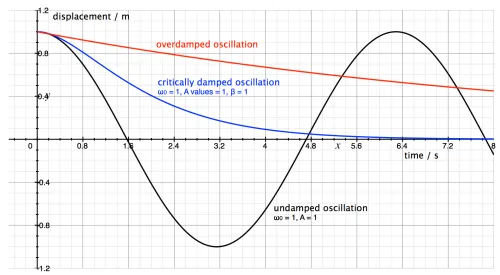
\includegraphics[width=0.8\textwidth]{Damping.png}
    \caption{Over Damping, Critical Damping, and Under Damping}
    \label{fig:Damping-png}
\end{figure}


\section{Forced Oscillation and Resonance}
\subsection{Definition}
\begin{definition}{Forced Oscillation}{}
    When a vibrating system is subjected to an external periodic force, the system is said to be under forced oscillation. \\
    The external periodic force is called the driving force, and the external agent is called a driver.
\end{definition}

\subsection{Differential Equation of Forced Oscillation}
The differential equation for damping harmonic motion can be written as \[
    \dv[2]{y}{t} + 2\lambda \dv{y}{t} + \omega^2 y = 0
\] Or, \[
    m \dv[2]{y}{t} + b \dv{y}{t} + ky = 0
\]

For forced oscillation, the differential equation is modified in the form
\begin{equation}
    m \dv[2]{y}{t} + b \dv{y}{t} + ky = F_0 \sin{\omega t}
\end{equation}

\subsection{Solution of the Differential Equation}
The general solution of the differential equation is
\begin{equation}
    \boxed{ y = y_h + y_p }
\end{equation}
Here, $y_h$ is the solution of the homogeneous equation, and $y_p$ is the particular integral of the non-homogeneous equation. \\
The solution of the homogeneous equation is
\begin{equation}
    \boxed{ y_h = A_1 e^{(-\lambda + \sqrt{\lambda^2 - \omega^2})t} + A_2 e^{(-\lambda - \sqrt{\lambda^2 - \omega^2})t} }
\end{equation}
Here, $A_1$ and $A_2$ are arbitrary constants. \\
The particular integral of the non-homogeneous equation is
\begin{equation}
    \boxed{ y_p = \frac{F_0}{m(\omega_0^2 - \omega^2)} \sin{\omega t} }
\end{equation}

Thus, the general solution of the differential equation is
\begin{equation}
    \boxed{ y = A_1 e^{(-\lambda + \sqrt{\lambda^2 - \omega^2})t} + A_2 e^{(-\lambda - \sqrt{\lambda^2 - \omega^2})t} + \frac{F_0}{m(\omega_0^2 - \omega^2)} \sin{\omega t} }
\end{equation}
Or,
\begin{equation}
    \boxed{ y = A_1 e^{-\lambda t} \sin{(\omega t + \theta)} + \frac{F_0}{m(\omega_0^2 - \omega^2)} \sin{\omega t} }
\end{equation}

\subsection{Resonance}
\begin{definition}{Resonance}{}
    The phenomenon of the increase in amplitude of oscillation of a system when the frequency of the driving force is equal to the natural frequency of the system is called resonance.
\end{definition}


\section{Wave Motion}
\subsection{Definition}
\begin{definition}{Wave}{}
    A wave is a disturbance that propagates through space and time, usually with transference of energy.
\end{definition}

\begin{definition}{Mechanical Wave}{}
    A mechanical wave is a wave that is an oscillation of matter, and therefore transfers energy through a medium.
\end{definition}

\begin{definition}{Electromagnetic Wave}{}
    An electromagnetic wave is a wave that is produced by oscillating electric charges and propagated by the periodic variation of intensities of, usually, perpendicular electric and magnetic fields.
\end{definition}

\subsection{Types of Waves}

\subsubsection{Mechanical Waves}
\begin{definition}{Transverse Wave}{}
    A transverse wave is a wave in which the particles of the medium vibrate perpendicular to the direction of propagation of the wave.
\end{definition}

\begin{definition}{Longitudinal Wave}{}
    A longitudinal wave is a wave in which the particles of the medium vibrate parallel to the direction of propagation of the wave.
\end{definition}

\begin{definition}{Progressive Wave}{}
    A progressive wave is a wave in which the particles of the medium vibrate in the same phase.
\end{definition}

\begin{definition}{Stationary Wave}{}
    A stationary wave is a wave in which the particles of the medium vibrate in the opposite phase.
\end{definition}

\subsubsection{Electromagnetic Waves}

\begin{definition}{Electromagnetic Wave}{}
    An electromagnetic wave is a wave that is produced by oscillating electric charges and propagated by the periodic variation of intensities of, usually, perpendicular electric and magnetic fields.
\end{definition}

\subsection{Equation of Motion}
Let $y$ be the displacement of a particle of a medium from its mean position at time $t$. \\

Then the equation of wave motion is
\begin{equation}
    \boxed{ y = r \sin{(\omega t - \varphi)} }
\end{equation}
Here, $r$ is the amplitude of the wave, $\omega$ is the angular frequency of the wave, and $\varphi$ is the phase of the wave. \\
We can also rewrite equation (7.3.1) substituting the values $\displaystyle \varphi = \frac{2\pi}{\lambda}x$, $\displaystyle \omega = \frac{2\pi}{T} = 2\pi n = \frac{2\pi}{\lambda} v$, and $\displaystyle k = \frac{2\pi}{\lambda}$, where $k$ is known as the propagation constant or the angular wave number. \\
Hence, equation (7.3.1) becomes
\begin{align*}
    y &= r \sin{\left( \omega t - \frac{2\pi}{\lambda}x \right)} \\
    y &= r \sin{\left( \frac{2\pi}{T}t - \frac{2\pi}{\lambda}x \right)}
\end{align*}
\begin{equation}
    \boxed{ y = r \sin{\frac{2\pi}{\lambda} \left( vt - x \right)} }
\end{equation}

Wave travelling in the negative $x$ direction:
\begin{equation}
    \boxed{ y = r \sin{\frac{2\pi}{\lambda} \left( vt + x \right)} }
\end{equation}

\subsection{Velocity, Slope, and Acceleration}
\subsubsection{Velocity of Wave and Velocity of Particle}
The velocity of the wave is given by
\begin{equation}
    \boxed{ v = \frac{\lambda}{T} = \lambda f = \frac{\omega}{k} }
\end{equation}

The velocity of the particle is given by
\begin{equation}
    \boxed{ V = \dv{y}{t} = \omega r \cos{(\omega t - \varphi)} = \frac{2\pi v}{\lambda} r \cos{\frac{2\pi}{\lambda}(vt - x)}}
\end{equation}

\subsubsection{Slope of the wave curve}
The slope of the wave curve is given by
\begin{equation}
    \boxed{ S = \dv{y}{x} = - \frac{2\pi}{\lambda} r \cos{\frac{2\pi}{\lambda}(vt - x)} }
\end{equation}

\subsubsection{Relation between Velocity and Slope}
From equations (7.4.2) and (7.4.3), we get
\begin{equation}
    \boxed{ \frac{V}{S} = -v }
\end{equation}
That is, \\
\begin{equation*}
    \boxed{ \text{Velocity of the particle} = - \text{Velocity of the wave} \times \text{Slope of the wave curve} }
\end{equation*}

\subsubsection{Acceleration of the particle}
The acceleration of the particle is given by
\begin{equation}
    \boxed{ A = \dv{V}{t} = - \frac{4\pi^2 v^2}{\lambda} r \sin{\frac{2\pi}{\lambda}(vt - x)} }
\end{equation}
Maximum acceleration,
\begin{equation}
    A_{\text{max}} = \frac{4\pi^2 v^2}{\lambda} r = 4\pi^2 f^2 r
\end{equation}

\subsection{Wave Packet, Phase Velocity, and Group Velocity}
\subsubsection{Definitions}
\begin{definition}{Wave packet}{}
    A wave packet is a short burst or envelope of localized wave action that travels as a unit. \\
    In other words, a wave packet is a group of waves consisting of slightly different frequencies superimposed upon each other.
\end{definition}

\begin{definition}{Phase velocity}{}
    The phase velocity is the velocity of each individual wave in the wave packet.
    \begin{equation}
        \boxed{ v_p = \frac{\omega}{k} = \frac{\omega\lambda}{2\pi} = \lambda f }
    \end{equation}
\end{definition}

\begin{definition}{Group velocity}{}
    The group velocity is the velocity of the wave packet.
    \begin{equation}
        \boxed{ v_g = \dv{\omega}{k} }
    \end{equation}
\end{definition}

\subsubsection{Relation between Phase Velocity and Group Velocity}
From equations (7.5.1) and (7.5.2), we get
\begin{align*}
    v_g &= \dv{\omega}{k} = \dv{(k v_p)}{k} \\
    &= v_p + k \dv{v_p}{k} \\
    &= v_p + k \dv{v_p}{\lambda} \dv{\lambda}{k} \\
    &= v_p + \frac{2\pi}{\lambda} \cdot \frac{1}{\dv{}{\lambda} \left( \frac{2\pi}{\lambda} \right)} \\
    &= v_p - \frac{2\pi}{\lambda}\frac{\lambda^2}{2\pi}\dv{v_p}{\lambda}
\end{align*}
\begin{equation}
    \boxed{ v_g = v_p - \lambda \dv{v_p}{\lambda} }
\end{equation}

\subsection{Differential Equation of Wave Motion}
Let $y$ be the displacement of a particle of a medium from its mean position at time $t$, and $x$ be the displacement of the particle from its mean position at time $t$. \\
Then we get,
\begin{equation}
    y = r \sin{\frac{2\pi}{\lambda}\left( vt - x \right)}
\end{equation}
\begin{equation*}
    \dv{y}{t} = \frac{2\pi v}{\lambda} r \cos{\frac{2\pi}{\lambda}\left( vt - x \right)}
\end{equation*}
\begin{equation}
    \boxed{ \dv[2]{y}{t} = -r \left( \frac{2\pi v}{\lambda} \right)^2 \sin{\frac{2\pi}{\lambda}\left( vt - x \right)} }
\end{equation}

From (7.6.1), we also get
\begin{equation*}
    \dv{y}{x} = - \frac{2\pi}{\lambda} r \cos{\frac{2\pi}{\lambda}\left( vt - x \right)}
\end{equation*}
\begin{equation}
    \boxed{ \dv[2]{y}{x} = \left( \frac{2\pi}{\lambda} \right)^2 r \sin{\frac{2\pi}{\lambda}\left( vt - x \right)} }
\end{equation}

From equations (7.6.2) and (7.6.3), we get
\begin{equation}
    \boxed{ \dv[2]{y}{t} = v^2 \dv[2]{y}{x} }
\end{equation}

\subsection{Energy Density and Energy Current (Intensity)}
\begin{definition}{Energy Density}{}
    Energy density is the total energy per unit volume passed through a medium
\end{definition}

\subsubsection{Kinetic Energy Density}
\begin{align*}
    \rho_K &= \frac{1}{2}(\text{mass density})(\text{velocity})^2 \\
    &= \frac{1}{2} \rho V^2 \\
    &= \frac{1}{2} \rho \left[ \frac{2\pi v}{\lambda} r \cos{\frac{2\pi}{\lambda} (vt - x)} \right]^2
\end{align*}
\begin{equation}
    \boxed{ \rho_K = \frac{1}{2} \rho \left( \frac{2\pi v}{\lambda} \right)^2 r^2 \cos^2{\frac{2\pi}{\lambda} (vt - x)} }
\end{equation}

\subsubsection{Potential Energy Density}
\begin{align*}
    \rho_U &= \int_{0}^{y} {\text{Force density} y} \: d{y} \\
    &= \int_{0}^{y} {(\text{mass density})(\text{acceleration}) y} \: d{y} \\
    &= \int_{0}^{y} {\rho \left[ \left(\frac{2\pi v}{\lambda}\right)^2 r \sin{\frac{2\pi}{\lambda}(vt-x)} \right] y} \: d{y}  \\
    &= \rho \left[ \left(\frac{2\pi v}{\lambda}\right)^2 r \sin{\frac{2\pi}{\lambda}(vt-x)} \right] \frac{y^2}{2}
\end{align*}
\begin{equation}
    \boxed{ \rho_U = \frac{1}{2} \rho \left( \frac{2\pi v}{\lambda} \right)^2 r^2 \sin^2{\frac{2\pi}{\lambda} (vt - x)} }
\end{equation}

\subsubsection{Total Energy Density}
From equations (7.7.1) and (7.7.2), we get the total energy density as \[
    \rho = \rho_K + \rho_U
\]
\begin{equation}
    \boxed{ \rho = \frac{1}{2} \rho \left( \frac{2\pi v}{\lambda} \right)^2 r^2 }
\end{equation}

\subsubsection{Energy Current (Intensity)}
\begin{definition}{Energy current}{}
    The ratio of flow of energy through unit cross-sectional area of the wave front along the direction of the wave propagation is knows as the Energy Current

    \begin{equation}
        \boxed{ C = \rho_E v = 2\pi^2f^2r^2\rho v }
    \end{equation}
\end{definition}

\begin{definition}{Intensity}{}
    The intensity is known as the incident energy per unit area of the wave front per unit time

    \begin{equation}
        \boxed{ I = 2\pi^2f^2r^2\rho v }
    \end{equation}
\end{definition}


\section{Stationary Wave}
\subsection{Definition}
\begin{definition}{Stationary Wave}{}
    When two exactly similar progressive wave trains travelling with the same velocity along the same straight line, but in opposite directions are superimposed upon each other, the resultant wave remains confined to the region in which it's produces, and is no more progressive. Such wave is known as stationary wave. \\
    In a nutshell, a stationary wave is a wave in which the particles of the medium vibrate in the opposite phase.
\end{definition}

\subsection{Stationary Waves in Vibrating Strings}
Let $y_1$ and $y_2$ be two progressive waves travelling in opposite directions. \\
Then, the equation of the two progressive waves are
\begin{align*}
    y_1 &= r \sin{\frac{2\pi}{\lambda}(vt - x)} \\
    y_2 &= - r \sin{\frac{2\pi}{\lambda}(vt + x)}
\end{align*}

Hence the equation of the stationary wave is
\begin{align*}
    y &= y_1 + y_2 \\
    &= r \sin{\frac{2\pi}{\lambda}(vt - x)} - r \sin{\frac{2\pi}{\lambda}(vt + x)} \\
    &= r \left[ \sin{\frac{2\pi}{\lambda}(vt - x)} - \sin{\frac{2\pi}{\lambda}(vt + x)} \right] \\
    &= 2r \cos{\left( \frac{2\pi}{\lambda}vt \right)} \sin{\left( -\frac{2\pi}{\lambda}x \right)}
\end{align*}
\begin{equation}
    \boxed{ y = - 2r \cos{\frac{2\pi}{\lambda}vt} \sin{\frac{2\pi}{\lambda}x} }
\end{equation}

Now, consider (8.2.1) be
\begin{equation}
    y = \left[ - 2r \cos{\frac{2\pi}{\lambda}vt} \right] \sin{\frac{2\pi}{\lambda}x}
\end{equation}

\begin{minipage}{0.45\textwidth}
    For zero amplitude:
    \begin{align*}
        \cos{\frac{2\pi}{\lambda}vt} &= 0 \\
        \frac{2\pi}{\lambda}vt &= \frac{\pi}{2}, \frac{3\pi}{2}, \frac{5\pi}{2}, \cdots \\
        \frac{2\pi t}{T} &= \left(n + \frac{1}{2}\right)\pi
    \end{align*}
    \begin{equation}
        \boxed{ t = \left( n + \frac{1}{2} \right) \frac{T}{2} }
    \end{equation}
\end{minipage}
\begin{minipage}{0.45\textwidth}
    For maximum amplitude:
    \begin{align*}
        \cos{\frac{2\pi}{\lambda}vt} &= \pm 1 \\
        \frac{2\pi}{\lambda}vt &= 0, \pi, 2\pi, \cdots \\
        \frac{2\pi t}{T} &= n\pi
    \end{align*}
    \begin{equation}
        \boxed{ t = n \frac{T}{2} }
    \end{equation}
\end{minipage}

\vspace{30pt}
Again, consider (8.2.1) be
\begin{equation}
    y = \left[ \sin{\frac{2\pi}{\lambda}x} \right] - 2r \cos{\frac{2\pi}{\lambda}vt}
\end{equation}

\begin{minipage}{0.45\textwidth}
    For maximum amplitude:
    \begin{align*}
        \sin{\frac{2\pi}{\lambda}x} &= \pm 1 \\
        \frac{2\pi}{\lambda}x &= \frac{\pi}{2}, \frac{3\pi}{2}, \frac{5\pi}{2}, \cdots \\
        \frac{2\pi}{\lambda} x &= \left( n + \frac{1}{2} \right) \pi
    \end{align*}
    \begin{equation}
        \boxed{ x = \left( n + \frac{1}{2} \right) \frac{\lambda}{2} }
    \end{equation}
\end{minipage}
\begin{minipage}{0.45\textwidth}
    For zero amplitude:
    \begin{align*}
        \sin{\frac{2\pi}{\lambda}x} &= 0 \\
        \frac{2\pi}{\lambda}x &= 0, \pi, 2\pi, \cdots \\
        \frac{2\pi}{\lambda} x &= n\pi
    \end{align*}
    \begin{equation}
        \boxed{ x = n \frac{\lambda}{2} }
    \end{equation}
\end{minipage}















\end{document}
